\section{Interpretació de l'enunciat i modelat de l'escenari}
En aquest apartat s'expliquen les extensions i suposicions de l'enunciat original,
així el modelat de l'entorn del robot.

Tal i com es demana el programa està parametritzat segons la posició de la càmera,
el punt P que aquesta detecta i l'angle $\alpha$. A més existeixen altres paràmetres
com els punts on es troben les peces originalment i on es deixen al final.

Per altra banda s'ha introduït la possibilitat de fixar un nombre diferent de peces
a cada pila, per tant es poden tenir piles amb diferent número de peces. També
és té amb compte la possibilitat de tenir més d'una peça, o cap, d'algun tipus.

Tots aquests paràmetres es tornen a veure detallats en l'apartat d'explicació del
codi on s'expliquen les \emph{Macros pròpies}\ref{macprop}.

En la figura \ref{escenari} següent es poden veure tots els paràmetres i punts
(marcats amb una estrella) que caracteritzen l'escenari.

\begin{figure}[H]
\begin{center}\label{fig:escenari}
 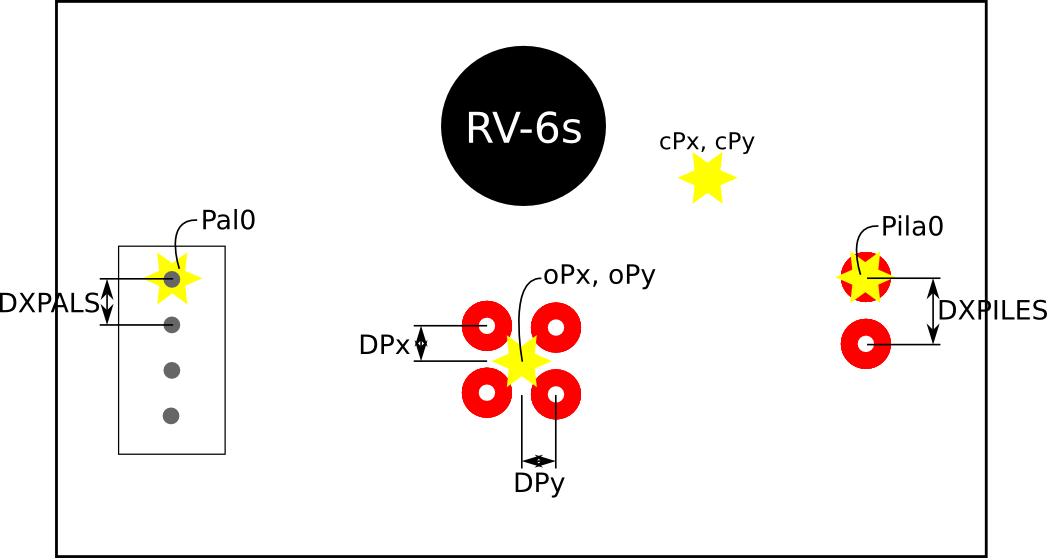
\includegraphics[width=0.8\textwidth]{escenari.png}
 % ordreRotacions.png: 1286x768 pixel, 150dpi, 21.77x13.00 cm, bb=0 0 617 369
\end{center}
  \caption{Escenari del robot}
\end{figure}

La figura es veu complementada amb el llistat de punts emprats a la pràctica.

\begin{minted}[frame=lines, fontsize=\small]{text}
DEF POS Paralisi = (337.16,  -14.95, 270.30, -179.98,  -0.36, -177.39)(7 ,0)
DEF POS Pal0     = (315.50, -550.72, 280.00, -173.00, -67.00,  -90.00)(7, 0)
DEF POS Pila0    = (337.18,  486.51, 280.00, -179.98,  -0.36,  -90.00)(7, 0)
DEF POS Pale0    = (  0.00,    0.00, 280.00, -179.98,  -0.36,  -90.00)(7, 0)
DEF POS PalePT   = (  0.00,    0.00, 280.00,  100.41,  85.49,   98.72)(6, 0)
DEF POS PaleOut0 = (337.00, -450.00, 280.00, -172.92, -66.76,  -90.00)(7, 0)
\end{minted}

Com es detalla en l'apartat de \emph{calcul de punts} \ref{calcpts}
s'ha intentat minimitzar el nombre de punts capturats per tal
de calcular els demes en realció a aquests.

A continuació s'explica l'utlitat de cada punt o posició.

\begin{description}
 \item [Paralisi] Guarda la posició del robot en repòs.
 \item [Pal0] Posició del primer pal (amb la pinça tombada).
 \item [Pila0] Posició de la primera pila (amb pinça perpendicular)
 \item [Pale0] Orientació del braç robot per posar peces del palé (amb la pinça
perpendicular).
 \item [PaleOut0] Orientació del braç robot per agafar les peces del palé
(amb la pinça tombada) 
\end{description}

L'enunciat deixa oberta la possibilitat de que fer amb les peces de
tipus 4, en aquest punt s'ha optat per posar-les al pal 4 per aprofitar el codi ja escrit i
així seguir la coherència i estructura dels tipus de peça anteriors. El fet de
no optar per apilar-les en qualsevol punt de l'entorn es perquè en la paletització
ja s'ha demostrat coneixement de com apilar peces i tractar el tipus 4 de manera
diferent als anteriors minvava elegància al codi i l'execució.

A efectes pràctics a la imatge següent es veu el posicionat de les peces de una forma
humanament comprensible emprant les marques fetes per els alumnes sobre l'entorn i existents
a data de \today. 

TODO FOTO peces sobre l'entorn.

A la imatge es pot apreciar com la primera pila esta al centre fet amb
rotulador negre i la segona seguint el cercle fet amb boli \emph{Bic} blau.

\section{Moviment del robot}
En aquest punt descrivim el moviment del braç robot i el perquè de l'ordre o
orientacions del mateix.

Totes les aproximacions a les peces es fan desde adalt. El braç robot es posiciona
a XY sobre la peça en qüestió i despés efectua un descens. Un cop agafada
efectua el moviment invers, ascens a Z i després el desplaçament corresponent
al pla XY on es conisderen segurs els moviments. Aquest pla de seguretat
en la practiva ve donat per la variable \texttt{ZS} fixada per defecte
a 280.0.

En primer lloc el robot agafa les peces del les piles inicials.
Aquestes són co\lgem ocades a la zona de paletització. Ambudes
accions és duen a terme amb la pinça perpendicular al plà XY, ja que es la
posició més segura i còmode de programar per l'agafada de peces.

Un cop acabat el muntatge del palé es desmunta amb la pinça tombada,
s'agafen les peces començant per les que es
troben més a l'esquerra del braç robot, per co\lgem ocarles als pals.

El fet de tombar la pinça és per incrementar l'abast del braç robot. Amb la
pinça perpendicular al pla XY, com s'havia efectuat el muntatge del palé, no
és possible arribar als pals 3 i 4. Com que s'ha decidit tombar la pinça
cap a l'esquerra\footnote{Com que els pals estan a la dreta del robot convé
tombar la pinça a la esquerra per simplificar els moviemnts i evitar haver
de fer un gir del braç}, desde el punt de vista del robot, s'han de recollir
les peces d'esquerra a dreta per tal de evitar que el braç co\lgem isioni
\ref{figcolisio} amb algun dels munts del palé encara existents.

\begin{figure}[H]
\begin{center}
 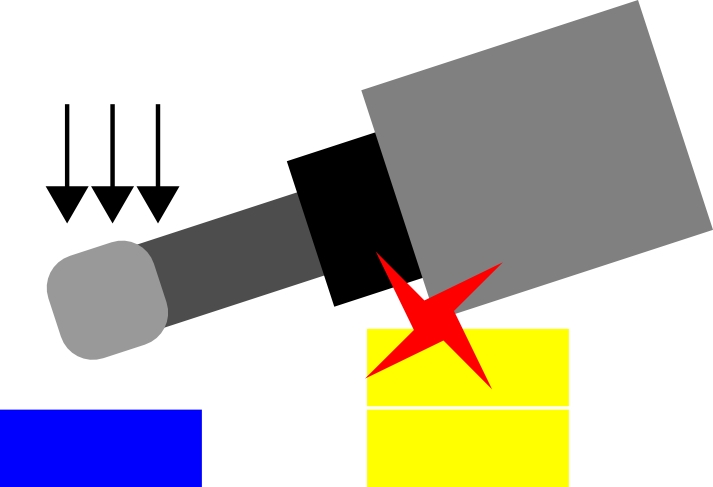
\includegraphics[width=0.6\textwidth]{colisio.png}
\end{center}
  \caption{Colisió amb el munt de peces grogues intentant agafar l'última peça blava}
\end{figure}\label{figcolisio}

Així doncs a la figura\ref{fig:recpec}
veim quin seria l'ordre de recollida depenent dels diferents angles per tal
d'evitar les possibles co\lgem isions.

\begin{figure}[H]
\begin{center}\label{figrecpec}
 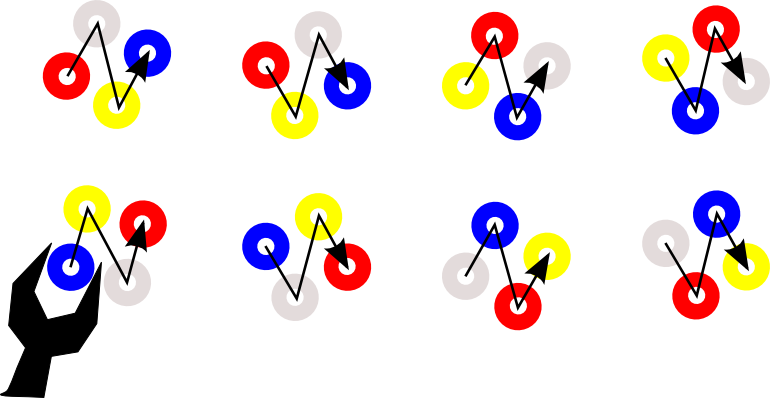
\includegraphics[width=0.8\textwidth]{ordreRotacions.png}
 % ordreRotacions.png: 1286x768 pixel, 150dpi, 21.77x13.00 cm, bb=0 0 617 369
\end{center}
  \caption{Ordre de recollida de les peces segons l'angle $\alpha$}
\end{figure}

Així doncs l'ordre de despaletització depèn de l'angle i no del tipus de peça.
Com és pot veure a la figura existeixen 8 possibles casos que es veuen
reflectits en l'explicació del codi font corresponent, secció \ref{casosrot}.